\section{Übertragungsmedien}
    \subsubsection{Kategorisierung Übertragungsmedien}
    \centering
    \includegraphics[width=0.8\linewidth]{images/Kategorisierung_übertragungsmedien.png}
    
    \subsubsection{Signale}
    \begin{theorem}{Ausbreitungsgeschwindigkeit}\\
        Funk- oder Licht-Signale sind elektromagnetische Wellen, die sich im Vakuum mit Lichtgeschwindigkeit $c_0 = 299'792'458$ ausbreiten. Die Vakuumgeschwindigkeit kann nicht überschritten werden.
        $$C_{Medium} = 200'000 km/s \approx 2/3 c_0$$
    \end{theorem}

    \begin{theorem}{Signaldämpfung}\\
        Die Signaldämpfung bezeichnet die Leistungsabnahme eines Signals auf einer Übertragungsstrecke. Die Angabe der Signaldämpfung erfolgt in dB als logarithmische Verhältniszahl von Eingangsleistung $P_1$ zur Aufgangsleistung $P_2$.
        $$Signaldämpfung[dB] = 10 \cdot log (\frac{P_1}{P_2}) = 10 \cdot log((\frac{U_1}{U_2})^2) = 20 \cdot log(\frac{U_1}{U_2})$$
        \includegraphics[width=1\linewidth]{images/Signaldämpfung.png}
    \end{theorem}    

    \begin{definition}{Dämpfungsbelag}\\
        Für Übertragungsmedien ist die Dämpfung pro Distanz massgebend. Typischerweise in dB pro 100 m angegeben. \\
        %\includegraphics[width=0.6\linewidth]{images/Dämpfungsbelag_Kabel.png}
    \end{definition}

    \begin{example2}{Berechnung Signaldämpfung/SNR}\\
        \includegraphics[width=0.75\linewidth]{images/example_signaldämpfung.png}
        $$U1/U2 = 1/0.5 = 2, Signaldämpfung = 20 \cdot log(2) = 6dB$$
    \end{example2}

    \subsection{Kabeltypen}
    \begin{concept}{Overview}
        \begin{itemize}
            \item Koaxialkabel: Geeignet für hochfrequente Signale
            \item Twinaxialkabel: Hoher Schutz (double koax)
            \item Twisted Pair (TP): Häufig im Einsatz (Shielded/Unshielded)
            \item Glasfaser: Hohe Bandbreite, Geringe Dämpfung, resistent
        \end{itemize}        
    \end{concept}

    \begin{definition}{Koaxialkabel}\\
        Eignen sich für hochfrequente Signale, unempfindlich gegenüber elektromagnetischen Störungen, früher Standard für Netzwerke, aber teuer und mechanisch heikel\\
            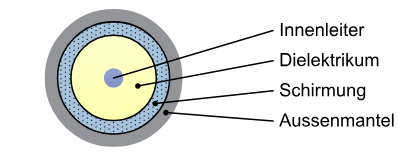
\includegraphics[width=0.3\linewidth]{images/Koaxkabel.png}
    \end{definition}

    \begin{definition}{Paarsymmetrische Kabel (Twisted Pair)}\\
        Häufig im Einsatz, auch für breitbandige Datenübertragung nutzbar, 
        Unterscheidung zwischen Shielded(STP)/Unshielded(UTP)
        \begin{itemize}
            \item Schirmeigenschaften
            \begin{itemize}
                \item Drahtgeflecht: niederfrequente Einstreuungen
                \item metallisch beschichtete Folien: hochfrequente Störungen
            \end{itemize}
            \item Bezeichnungsschema ISO/IEC 11801\\
            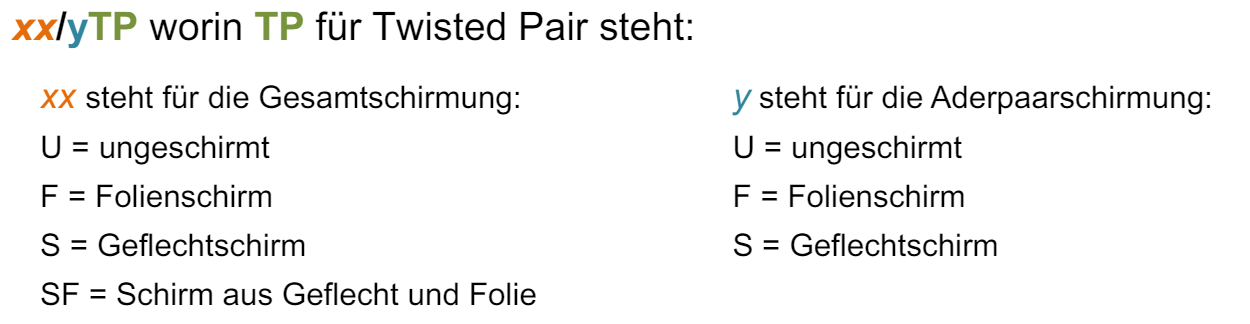
\includegraphics[width=\linewidth]{images/STP_Schirmeigenschaften.png}
        \end{itemize}
        Anfälliger auf Störungen (crosstalk), kapazitiv oder induktiv, Methoden zur Behebung:
        \begin{itemize}
            \item Kapazitiv: Komplementäres Signal, elektrisch leitenden Schirm
            \item Induktiv: Verdrillte Aderpaare
        \end{itemize}
    \end{definition}

    \begin{concept}{Lichtwellenleiter}\\
        Hohe Bandbreite, Geringe Dämpfung, Resistent, Dispersion als begrenzender Faktor
        \begin{comment}
              \begin{itemize}
            \item Zentrum aus Kernglas mit hoher optischer Dichte (Brechungsindex 1.5)
            \item Vom Mantelglas umschlossen, geringere optische Dichte (Brechungsindex 1.48)
        \end{itemize}
            \centering
            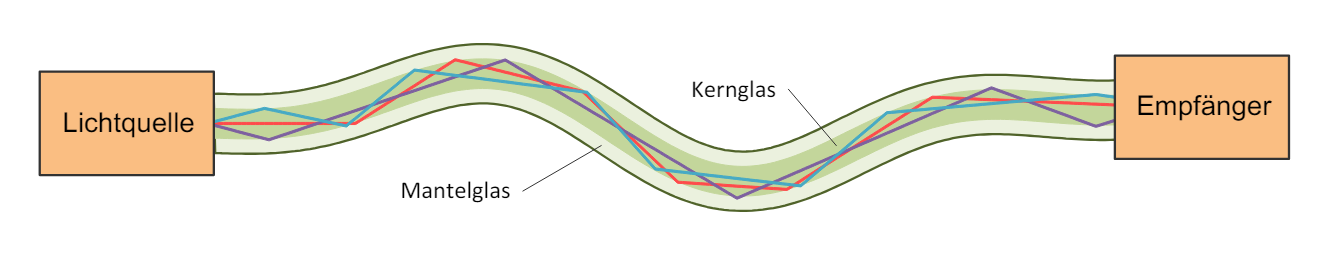
\includegraphics[width=1\linewidth]{images/Lichtwellenleiter.png}\\
        \end{comment}
        \begin{itemize}
            \item Multimode: dicker Kern, günstiger, kleinere Datenraten und Übertragungsstrecken
            \begin{itemize}
                \item Stufenfasern
                \item Gradientenfasern
            \end{itemize}
            \item Singlemode: dünner Kern, teuer!! aber funktionieren super
        \end{itemize}
        \vspace{2mm}
        \textbf{Grundprinzip optischer Fasern beruht auf der Totalreflexion und der Ausbreitung des Lichtes in bestimmten Moden}
    \end{concept}

    \begin{KR}{Key Takes}
        \begin{itemize}
            \item Halbierung der Leistung entspricht ca. 3dB
            \item für SNR gleiche Formel wie Signaldämpfung, aber $P_1 = P_{Signal}$ und $P_2 = P_{Störung}$
            \item Entscheidend für die maximale Leitungslänge sind Dämpfungsbelag und SNR
            \item senkt man die Bitrate (Bit/s) können grössere Distanzen erreicht werden
            \item Die Bandbreite (Frequenz) ist in der Grafik abhängig zum Dämpfungsbelag.
            \item Die höheren Kabelkategorien brauchen, um höhere Dämpfung zu tolerieren, bessere Schirmungen, um das Übersprechen zu minimieren.
        \end{itemize}
    \end{KR}

    

    \subsubsection{Strukturierte Gebäudeverkabelung nach ISO/IEC 11801}
        \centering
        \includegraphics[width=1\linewidth]{images/Gebäudeverkabelung.png}
        
    